\documentclass[12pt]{article}
\usepackage[a4paper, margin=.30in]{geometry}
\usepackage{array}
\usepackage{fancybox}
\usepackage{amsmath,amsfonts,amssymb}
\usepackage{graphicx}
\usepackage{array}
\usepackage{booktabs}
\usepackage{xcolor}
\usepackage{pgfplots}
\usepackage{multirow}
\usepackage{tikz}
\usepackage{float}
\usepackage{hyperref}
\usepackage{subfig, wrapfig, makecell}
\usepackage{pgf-pie}
\newcommand\headerMe[2]{\noindent{}#1\hfill#2}
\renewcommand \thesection{\Roman{section}}

\newcolumntype{M}[1]{>{\raggedright}m{#1}}

\usepackage{tikz}


\begin{document}

\headerMe{Royaume du Maroc}{année scolaire \emph{2024-2025}}\\
\headerMe{Ministère de l'Éducation nationale, }{  Professeur :\emph{Zakaria Haouzan}}\\
\headerMe{du Préscolaire et des Sports}{Établissement : \emph{Lycée SKHOR qualifiant}}\\

\begin{center}
Devoir surveillé N°1 \\
Durée 2h00\\
\underline{2-BAC Section des sciences expérimentales: Option de sciences physiques}\\

    \vspace{.2cm}
\hrulefill
\Large{Fiche Pédagogique}
\hrulefill\\
\end{center}
%end Headerss------------------------


%__________________Chimie ______________________-
%%%%%%%+_+_+_+_+_+_+_+_+_Partie1
\section[A]{Introduction }
\hspace{0.5cm}Le programme d'études de la matière physique chimie vise à croître un ensemble de compétences visant à développer la personnalité de l'apprenant. Ces compétences peuvent être classées en Compétences transversales communes et Compétences qualitatives associées aux différentes parties du programme.
\section{cadre de référence }
 \hspace{0.5cm}L'épreuve a été réalisée en adoptant des modes proches à des situations d'apprentissages et des situations problèmes, qui permettent de compléter les connaissances et les compétences contenues dans les instructions pédagogiques et dans le programme de la matière physique chimie et aussi dans le cadre de référence de l'examen national. 
 \\Tout en respectant les rapports d'importance précisés dans les tableaux suivants :
 \begin{center}
\begin{tabular}{|c||c||c|}
\hline
    \textbf{Restitution des Connaissances} & \textbf{Application des Connaissances} & \textbf{Situation Problème }\\
    \hline 
    $50\%$ & $25\%$ & $25\%$\\
    \hline
\end{tabular} 
\end{center}

\section{tableau de spécification}
 \begin{center}
\begin{tabular}{||c|c||c|c|c|c|}
\hline
     \multicolumn{2}{||c||}{\bf{   \hfill  Niveau d'habileté  \hfill } }
	& \makecell{Restitution \\des Connaissances} &\makecell{Application \\des Connaissances} & \makecell{Situation Problème} & la somme \\\hline

	%  
\multirow{1}{*}{ Les Ondes 53\%}
	& \makecell{Les Ondes\\mécaniques\\progressives}  & \makecell{6,5\%\\1Q - 0,5pts}  &\makecell{3,25\%\\1Q - 1pt} & \makecell{3,25\%\\} & 

	\multirow{3}{*}{\makecell{53\%\\13pts\\14Q\\65min}}\\\cline{2-5}
& \makecell{Les Ondes \\périodiques}  & \makecell{10\%\\1Q - 0,5pts}  &\makecell{5\%\\1Q - 1pt } & \makecell{5\%\\2Q - 1pt} &\\\cline{2-5}

& \makecell{Les Ondes \\lumineuse}  & \makecell{10\%\\4Q - 3pts}  &\makecell{5\%\\5Q - 4pt } & \makecell{5\%\\1Q - 2pt} &\\\hline

\multirow{2}{*}{ \makecell{Les\\Transformations\\d'un\\système\\chimique 47\%}}

& \makecell{lentes\\et\\rapides}  & \makecell{\\4\%\\3Q - 2.5pts}  &\makecell{2\% } & \makecell{1\%} &

\multirow{1}{*}{\makecell{47\%\\7pts\\12Q\\55min }}\\\cline{2-5}

& \makecell{Suivi\\temporel}  & \makecell{\\20\%\\1Q - 0,5pts}  &\makecell{\\10\%\\1Q - 0,5pts } & \makecell{\\10\%\\2Q - 1,25pts} &\\\hline



     \multicolumn{2}{||c||}{\bf{   \hfill  --  \hfill } }
& \makecell{50\%\\13Q - 11pts}  &\makecell{25\%\\6Q - 4,5pts } & \makecell{25\%\\8Q - 4,5pts} &\\\hline



\end{tabular} 
\end{center}

\newpage
\begin{center}
    \shadowbox{\bf{ Devoir surveillé $N^{\circ}$1 Semestre I} }
\end{center}
 \begin{center}

     \begin{tabular}{|c||c||c|}
    \hline
         \multicolumn{3}{||c||}{\bf{   \hfill  Chimie  \hfill (7pts)} }\\
         \hline
         \multicolumn{3}{||c||}{\bf{Suivi temporel d’une transformation chimique\dotfill} }\\
\hline
    \textbf{$N^{\circ}$Q. } & \textbf{Réponse } & \textbf{Note }\\
    \hline
    $1.$ &
         \makecell{les quantités de matière initiales des réactifs.\\
       $n_0(CaCO_{3(s)}) = 3.10^{-3} mol$ et $n_0(H_3O^+_{(aq)}) = 5.10^{-3}mol$
 }
    & $1pts$\\\hline
 %Q2
     $2.$ &
     \makecell{
		 le tableau d’avancement de cette réaction.\\
 \begin{tabular}{|c|c|c|c|c|c|c|}
    \hline
	\multicolumn{2}{|c|}{Equation de la réaction}& \multicolumn{5}{c|}{$2H_3O^+$ + $CaCO_3$ $\rightarrow$ $Ca^{2+}$ + $CO_2$ + $3H_2O$}\\\hline
    états  & avancement& \multicolumn{5}{|c|}{quantité de Matière en mol}\\\hline
    Etat initial          &    0        &  0,04&0,01&  0              &  0 & 0 \\\hline
   \makecell{Etat de \\transformation}&$x$ & $0,04-2x$ & $ 0,01-x$ & $x$  & $x$ & $x$ \\\hline
    Etat final&    $x_{max}$& $ 0,04 - 2x_{max}$ & $0,01 - x_{max}$ & $2x_{max}$  & $x_{max}$ & $x_{max}$ \\\hline
   % \cline{2-4}\
\end{tabular}\\
	 }
    & $0,5pts$\\\hline  
 %Q3
     $3$ &
       \makecell{ $x_{max} = 10^{-3}mol$ et le réactif limitant $H_3O^+$.}
    & $1pts$\\\hline  
 %Q4
     $4$ &
         \makecell{ Montrer que $V(CO_2) = 2,44.10^{-2}.x$}
    & $0.5pt$\\\hline  
 %Q5
     $5$ &
       \makecell{Montrer que $V(CO_2)_{t1/2} = 25mL $ et $t_{1/2} = 75s$}
    & $0,75pt$\\\hline  
	 $6$ &
       \makecell{la vitesse volumique de la réaction à l’instant de date t = 0 $V(t=0) = 0,24 mol/L.s$}
    & $0,5pts$\\\hline  

    $7$ &
	\makecell{La valeur du temps de
demi- réaction est inférieure à la valeur précédente }
    & $0,5pt$\\\hline  
     \multicolumn{3}{||c||}{\bf{Partie 2 : Mesure de conductivité \dotfill (2,25pts)} }\\
\hline
    \textbf{$N^{\circ}$Q } & \textbf{Réponse } & \textbf{Note }\\
    \hline
    $1$ &
         \makecell{ conductivité du mélange réactionnel à l’état initial.\\ $\sigma_i = \lambda_{H_3O^+}[H_3O^+] + \lambda_{Cl^-}[Cl^-] = 0,8526S/m$}
    & $0,75pt$\\\hline
 %Q2
 $2$ &
         \makecell{Montrer que l’avancement : $\sigma =-580.x(t) + \sigma_i$ }
    & $0,5pt$\\\hline
 %Q3
 $3$ &
         \makecell{Montrer que la vitesse volumique $v(t)= -17,2.\frac{d\sigma(t)}{dt}$ }
    & $1pt$\\\hline
      %Partie 2 : -----


%%Partie 2 : 
         %\multicolumn{3}{||c||}{\bf{Partie 2 : Suivi d’une transformation chimique\dotfill (2pts)}}\\
%\hline
%$1.$ &
         %\makecell{\\ % table dont forget 
             %\begin{tabular}{|c|c|c|c|c|c|}
    %\hline
    %\multicolumn{2}{|c|}{Equation de la réaction}& \multicolumn{4}{c|}{2CuO + C $\rightarrow$ 2Cu + $CO_2$}\\\hline
    %états  & avancement& \multicolumn{4}{|c|}{quantité de Matière en mol}\\\hline
    %Etat initial          &    0        &  12.38 &  1.4&  0              &  0 \\\hline
                 %\makecell{Etat de \\transformation}&    $x$      & $ 12.38 - 2x$ & $ 1.4 - x$ & $ 2x$  & $x$ \\\hline
    %Etat final            &    $x_{max}$& $ 12.38 - 2x_{max}$ & $1.4 - x_{max}$ & $2x_{max}$  & $x_{max}$ \\\hline
   %% \cline{2-4}\
%\end{tabular}
         %\\$\; $ }  
    %& $1pt$\\\hline
 %%Q2
   %$2$ &
         %\makecell{ l’avancement maximal $x_{max} = 1.4mol$ et le réactif limitant le carbone C(s) 
 %}
    %& $0.5pt$\\\hline  
 %%Q3
   %$3$ &
         %\makecell{ bilan de matière dans l’état final :\\ $n_f(CuO) = 9.58 mol$ et $n_f(C) = 0 mol$ et $n_f(Cu) = 2.8 mol$, $n_f(CO_2) = 1.4mol$ 
 %}
    %& $0.5pt$\\\hline  
%Physique : 
    %Partie 1 : 
\end{tabular} 
\end{center}

\begin{center}
  \begin{tabular}{|c||c||c|}
    \hline
         \multicolumn{3}{||c||}{\bf{   \hfill  Physique  \hfill (13pts)} }\\
         \hline
         \multicolumn{3}{||c||}{\bf{Partie 1 : le mouvement des vagues \dotfill (3pts)} }\\
\hline
    \textbf{$N^{\circ}$Q.} & \textbf{Réponse } & \textbf{Note }\\
    \hline
    $1$ &
         \makecell{
			 L’onde étudiée est transversale}
    & $0,5pt$\\\hline
 %Q2
 $2$ &
         \makecell{ la courbe représentant l’élongation du
point M. courbe 1}
    & $0,5pt$\\\hline
 %Q3
 $3$ &
         \makecell{
            Par exploitation des courbes précédentes, :\\
            $\tau = 8.10^{-2}s$ et $t_1 = 24.10^{-2}s$;\\
            $d = 26.10^{-2}m$ car $v = \frac{80.10^{-2}}{24.10^{-2}} = 3,33m/s$
      }
    & $2pt$\\\hline
 %Q3
 $3$ &
         \makecell{
           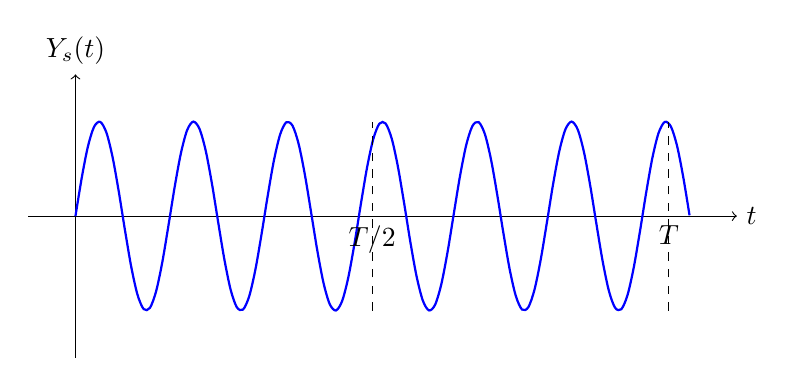
\begin{tikzpicture}[scale=1.2]
    \draw[->] (-0.5,0) -- (7,0) node[right] {\(t\)}; % Time axis
    \draw[->] (0,-1.5) -- (0,1.5) node[above] {\(Y_s(t)\)}; % Elongation axis
    % Sine wave
    \draw[thick,blue,domain=0:6.5,samples=100,smooth] 
        plot (\x,{sin(2*3.14159*\x r)});
    % Labels
    \node at (3.14,0) [below] {\(T/2\)};
    \node at (6.28,0) [below] {\(T\)};
    \draw[dashed] (3.14,-1) -- (3.14,1);
    \draw[dashed] (6.28,-1) -- (6.28,1);
\end{tikzpicture}
    }
    & $0,5pt$\\\hline
%1
 $1$ &
    \makecell{Montrer que $\lambda' = \sqrt{2}.\lambda$ }
    & $0,5pt$\\\hline

     \multicolumn{3}{||c||}{\bf{Partie 2 : Étude du phénomène ondulatoire.\dotfill (5pts)} }\\
\hline
%1
 $1$ &
 \makecell{Nom du phénomène observé diffraction la nature de
la lumière monochromatique }
    & $1pt$\\\hline
%2
 $2$ &
 \makecell{a l’aide de la figure 1 $\theta = \frac{L}{2.D}$ }
    & $0,5pt$\\\hline
 $3$ &
 \makecell{En utilisant les résultats des mesures $\theta = 3,15.10^{-3} rad$ }
    & $0,5pt$\\\hline

 $4$ &
 \makecell{la relation qui lie les grandeurs  $\theta = \frac{\lambda}{a}$ 
}
 
    & $0,5pt$\\\hline
 $5$ &
 \makecell{la valeur de la longueur d'onde  $\lambda = 0,63m$ \\elle appartient au domaine visible 
}
 & $0,5pt$\\\hline

 $6$ &
 \makecell{-on remplace la lumière émise par le LASER (lumière rouge) par une lumière bleue\\L diminue\\
	 -n diminue la largeur de la fente a L augmente\\
	 -différencier expérimentalement une lumière monochromatique d’une lumière \\ polychromatique  par un prisme
}
 & $2pt$\\\hline

  \end{tabular}
  \end{center}
\newpage

\section{Introduction}

Ce document présente une analyse détaillée des résultats obtenus par les élèves lors du Devoir Surveillé N°1 en sciences physiques. L'examen, d'une durée de 2 heures, était divisé en deux parties principales : la chimie (7 points) et la physique (13 points). Cette analyse vise à identifier les forces et les faiblesses des élèves, ainsi qu'à proposer des stratégies d'amélioration pour les prochaines séquences d'apprentissage.

\section{Analyse Statistique des Résultats}

\subsection{Distribution des Notes}

L'analyse porte sur un effectif de 36 élèves ayant passé l'examen. Voici les principales statistiques concernant les résultats obtenus :

\begin{center}
\begin{tabular}{|l|c|}
\hline
\textbf{Statistique} & \textbf{Valeur} \\
\hline
Note minimale & 1,00 /20 \\
Note maximale & 16,50 /20 \\
Moyenne de la classe & 7,81 /20 \\
Médiane & 8,25 /20 \\
Écart-type & 4,48 \\
\hline
\end{tabular}
\end{center}

\subsection{Visualisation de la Distribution}

\begin{figure}[H]
\centering
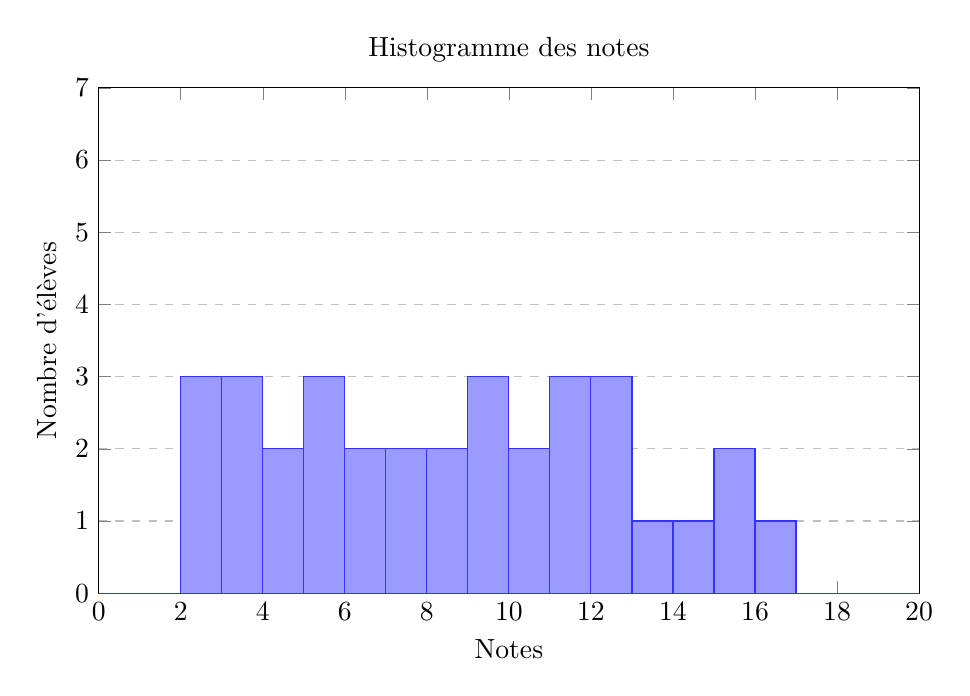
\begin{tikzpicture}
\begin{axis}[
    xlabel={Notes},
    ylabel={Nombre d'élèves},
    ymin=0, ymax=7,
    xmin=0, xmax=20,
    width=12cm,
    height=8cm,
    ymajorgrids=true,
    grid style=dashed,
    title={Histogramme des notes},
]
\addplot[ybar interval,fill=blue!40,draw=blue!80] 
    coordinates {(0,0) (1,0) (2,3) (3,3) (4,2) (5,3) (6,2) (7,2) (8,2) (9,3) (10,2) (11,3) (12,3) (13,1) (14,1) (15,2) (16,1) (17,0) (18,0) (19,0) (20,0)};
\end{axis}
\end{tikzpicture}
\caption{Distribution des notes des élèves}
\end{figure}

\subsection{Répartition des Notes par Intervalles}

\begin{center}
\begin{tabular}{|l|c|c|}
\hline
\textbf{Intervalle de notes} & \textbf{Nombre d'élèves} & \textbf{Pourcentage} \\
\hline
{[}0 - 5{[} & 11 & 30,56\% \\
{[}5 - 10{[} & 12 & 33,33\% \\
{[}10 - 15{[} & 10 & 27,78\% \\
{[}15 - 20{]} & 3 & 8,33\% \\
\hline
\end{tabular}
\end{center}

\begin{figure}[H]
\centering
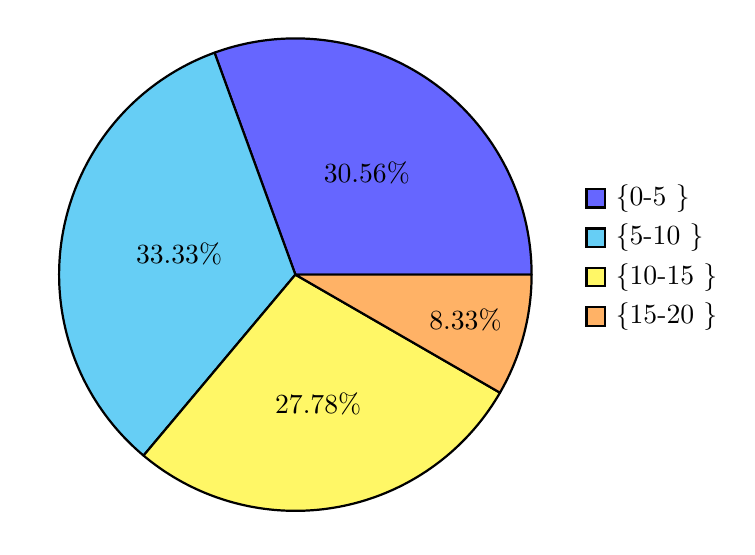
\begin{tikzpicture}
%\pie[text=legend]{30.56/{[}0-5{[}}, 33.33/{[}5-10{[}}, 27.78/{[}10-15{[}}, 8.33/{[}15-20{]}}
\pie[text=legend]{
  30.56/{\textbraceleft 0-5 \textbraceright}, 
  33.33/{\textbraceleft 5-10 \textbraceright}, 
  27.78/{\textbraceleft 10-15 \textbraceright}, 
  8.33/{\textbraceleft 15-20 \textbraceright}
}
\end{tikzpicture}
\caption{Répartition des notes par intervalles}
\end{figure}

\subsection{Taux de Réussite}

\begin{itemize}
\item \textbf{Taux de réussite} (note $\geq$ 10/20) : 36,11\% (13 élèves)
\item \textbf{Taux d'échec} (note $<$ 10/20) : 63,89\% (23 élèves)
\end{itemize}

\begin{figure}[H]
\centering
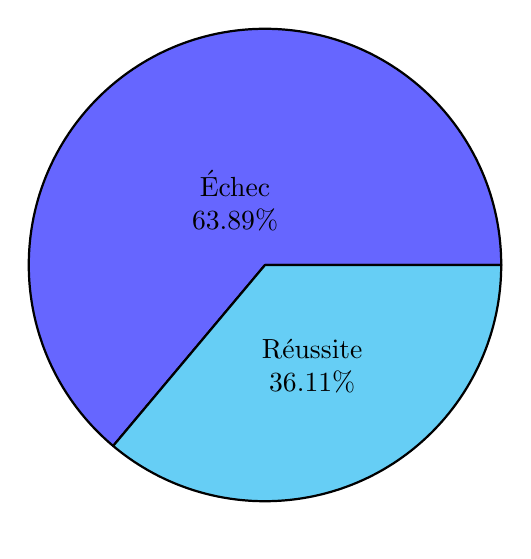
\begin{tikzpicture}
\pie[text=inside]{63.89/Échec, 36.11/Réussite}
\end{tikzpicture}
\caption{Répartition réussite/échec}
\end{figure}

\section{Analyse par Partie du Devoir}

\subsection{Performance Comparative Chimie/Physique}

En normalisant les résultats sur une base de 10 points pour faciliter la comparaison :

\begin{center}
\begin{tabular}{|l|c|c|}
\hline
\textbf{Partie} & \textbf{Moyenne /10} & \textbf{Taux de réussite} \\
\hline
Chimie (7 pts) & 3,91 /10 & 32,14\% \\
Physique (13 pts) & 4,25 /10 & 38,89\% \\
\hline
\end{tabular}
\end{center}

\begin{figure}[H]
\centering
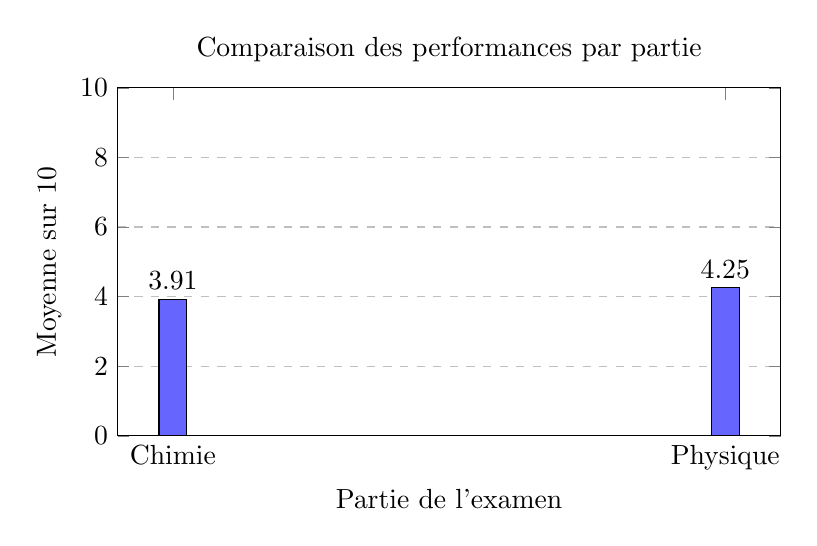
\begin{tikzpicture}
\begin{axis}[
    xlabel={Partie de l'examen},
    ylabel={Moyenne sur 10},
    ymin=0, ymax=10,
    symbolic x coords={Chimie, Physique},
    xtick=data,
    width=10cm,
    height=6cm,
    ymajorgrids=true,
    grid style=dashed,
    title={Comparaison des performances par partie},
    nodes near coords,
]
\addplot[ybar,fill=blue!60] coordinates {(Chimie, 3.91) (Physique, 4.25)};
\end{axis}
\end{tikzpicture}
\caption{Comparaison des moyennes par partie}
\end{figure}

\subsection{Analyse par Compétence}

\begin{center}
\begin{tabular}{|l|c|}
\hline
\textbf{Niveau d'habileté} & \textbf{Performance moyenne} \\
\hline
Restitution des Connaissances & 52,43\% \\
Application des Connaissances & 39,67\% \\
Situation Problème & 31,25\% \\
\hline
\end{tabular}
\end{center}

\begin{figure}[H]
\centering
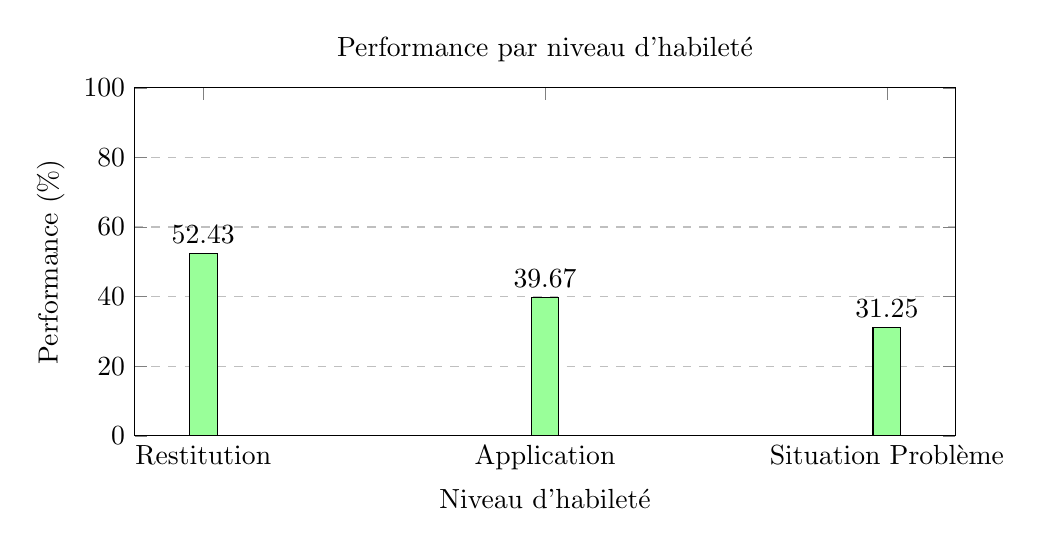
\begin{tikzpicture}
\begin{axis}[
    xlabel={Niveau d'habileté},
    ylabel={Performance (\%)},
    ymin=0, ymax=100,
    symbolic x coords={Restitution, Application, Situation Problème},
    xtick=data,
    width=12cm,
    height=6cm,
    ymajorgrids=true,
    grid style=dashed,
    title={Performance par niveau d'habileté},
    nodes near coords,
]
\addplot[ybar,fill=green!40] coordinates {(Restitution, 52.43) (Application, 39.67) (Situation Problème, 31.25)};
\end{axis}
\end{tikzpicture}
\caption{Performance par niveau d'habileté}
\end{figure}

\section{Identification des Difficultés Principales}

\subsection{En Chimie}

\subsubsection{Points forts}
\begin{itemize}
\item Calcul des quantités de matière initiales
\item Identification du réactif limitant
\end{itemize}

\subsubsection{Difficultés majeures}
\begin{itemize}
\item Établissement de la relation entre conductivité et avancement
\item Expression de la vitesse volumique en fonction de la conductivité
\item Interprétation de l'influence de la température sur la cinétique
\end{itemize}

\subsection{En Physique}

\subsubsection{Points forts}
\begin{itemize}
\item Identification des ondes transversales
\item Calcul de l'angle de diffraction
\end{itemize}

\subsubsection{Difficultés majeures}
\begin{itemize}
\item Exploitation des graphiques pour déterminer les paramètres d'une onde
\item Calcul de l'indice de réfraction du prisme
\item Analyse des phénomènes de dispersion de la lumière
\end{itemize}

\section{Recommandations Pédagogiques}

\subsection{Remédiation Immédiate}
\begin{itemize}
\item Organiser une séance de correction détaillée du devoir avec explication des erreurs fréquentes
\item Fournir des exercices supplémentaires ciblant les points faibles identifiés
\end{itemize}

\subsection{Ajustements pour l'Enseignement Futur}

\subsubsection{En Chimie}
\begin{itemize}
\item Renforcer les activités pratiques sur la cinétique chimique
\item Travailler davantage sur l'interprétation physique des équations et des relations
\item Proposer des exercices combinant plusieurs méthodes de suivi (conductimétrie, pH-métrie, etc.)
\end{itemize}

\subsubsection{En Physique}
\begin{itemize}
\item Accentuer le travail sur l'interprétation graphique des phénomènes ondulatoires
\item Proposer des activités expérimentales sur la diffraction et la dispersion
\item Renforcer l'exploitation mathématique des résultats d'expérience
\end{itemize}

\subsection{Différenciation Pédagogique}
\begin{itemize}
\item Former des groupes de travail mixtes (élèves en difficulté avec élèves plus avancés)
\item Proposer des exercices à difficulté progressive pour chaque niveau d'habileté
\item Offrir des séances de soutien ciblées pour les élèves ayant obtenu moins de 5/20
\end{itemize}

\section{Conclusion}

L'analyse des résultats du Devoir Surveillé N°1 révèle un taux de réussite globalement insuffisant (36,11\%), avec une moyenne de classe de 7,81/20. Les difficultés les plus importantes concernent les situations-problèmes et l'application des connaissances, particulièrement dans les domaines de la cinétique chimique et des phénomènes ondulatoires complexes.

Il est recommandé de renforcer l'approche expérimentale et de multiplier les situations d'application concrète des concepts théoriques. La mise en place d'une pédagogie différenciée et d'un suivi plus personnalisé des élèves en difficulté devrait permettre d'améliorer les résultats lors des prochaines évaluations.

\end{document}
